\section{1174077 - Alvan Alvanzah}
\subsection{Teori}
\subsubsection{Jelaskan Apa Itu Binary Classification dilengkapi ilustrasi gambar sendiri.}

Klasifikasi biner bertujuan untuk mengklasifikasikan elemen-elemen dari himpunan yang diberikan ke dalam dua kelompok (memprediksi kelompok mana yang masing-masing dimiliki) berdasarkan aturan klasifikasi. 
\hfill\\
\begin{figure}[H]
    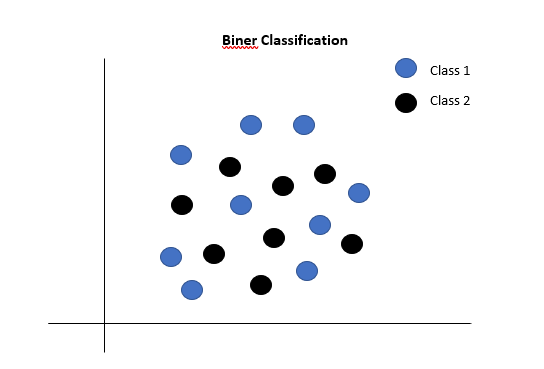
\includegraphics[width=12cm]{figures/1174077/2/kb.png}
    \centering
    \caption{Binary Classification}
\end{figure}

\subsubsection{Jelaskan Apa itu supervised learning , unsupervised learning dan clusterring dengan ilustrasi gambar sendiri.}
\begin{enumerate}
\item supervised learning
\hfill\\
Supervised learning adalah suatu pembelajaran yang terawasi dimana output yang diharapkan telah diketahui sebelumnya. Biasanya pembelajaran ini dilakukan dengan menggunakan data yang telah ada. Dan Supervised Learning dalam bahasa indonesia adalah pembelajaran yang ada supervisornya. Maksudnya  ada supervisornya adalah label di tiap data nya. 
\begin{figure}[H]
    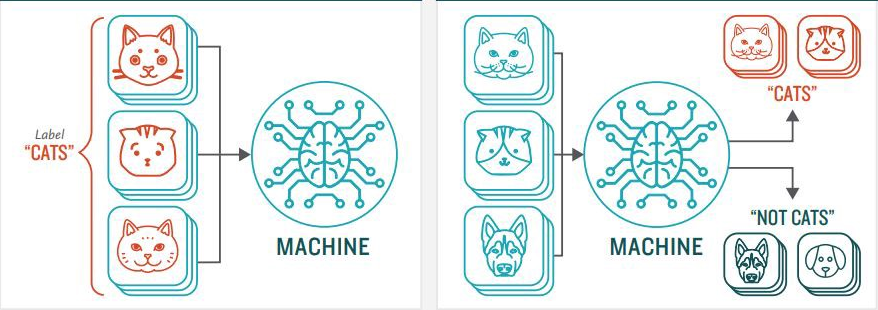
\includegraphics[width=12cm]{figures/1174077/2/sl.png}
    \centering
    \caption{Supervised Learning}
\end{figure}

\item unspervised learning
\hfill\\
Unsupervised learning berbeda dengan supervised learning. Unsupervised learning memiliki keunggulan dari supervised learning. Supervised learning memiliki label sebagai dasar prediksi untuk membuat clasification dan regression algorithm yang memungkinkan. Tetapi dalam realitanya, data real banyak yang tidak memiliki label. Jadi unsupervised learning menggunakan ke samaan dari attribut attribut yang dimiliki untuk mencari kemiripan,dan kemudian dikelompok kelompokan (clustering). Sehingga hal ini akan menimbulkan kelompok kelompok (cluster). 
\begin{figure}[H]
    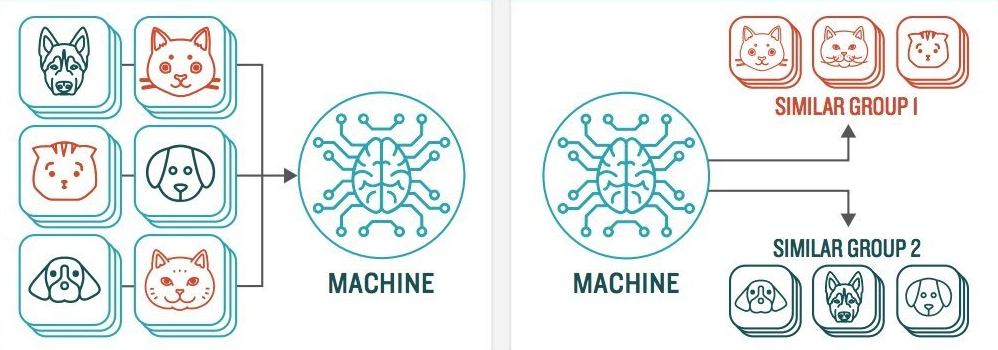
\includegraphics[width=12cm]{figures/1174077/2/ul.png}
    \centering
    \caption{Unsupervised Learning}
\end{figure}

\item Clustering 
\hfill\\
Clustering adalah sebuah metode untuk mengkelompokan data - data menjadi kumpulan dari group yang isinya merupakan data yang serupa setiap grupnya. Basisnya dapat berupa kesamaan atau perbedaan attribut dari setiap grup tersebut.
\begin{figure}[H]
    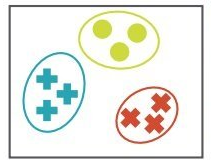
\includegraphics[width=12cm]{figures/1174077/2/cl.png}
    \centering
    \caption{gambaran clustering}
\end{figure}
\end{enumerate}

\subsubsection{Jelaskan apa itu evaluasi dan akurasi dan disertai ilustrasi contoh dengan gambar sendiri}
\hfill\\
Evaluasi adalah tentang bagaimana kita dapat mengevaluasi seberapa baik model bekerja dengan mengukur akurasinya. Dan akurasi akan didefinisikan sebagai persentase kasus yang diklasifikasikan dengan benar. Kita dapat menganalisis kesalahan yang dibuat oleh model,atau tingkat kebingungannya,menggunakan matriks kebingungan. 
\begin{figure}[H]
    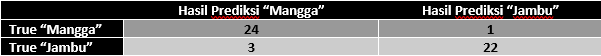
\includegraphics[width=12cm]{figures/1174077/2/ea.png}
    \centering
    \caption{Evaluasi dan Akurasi}
\end{figure}

\subsubsection{Jelaskan bagaimana cara membuat Confusion Matrix, Buat confusion matrix sendiri.}
\hfill\\
Confusion Matrix suatu metode yang biasanya digunakan untuk melakukan perhitungan akurasi pada konsep data mining atau Sistem Pendukung Keputusan. Pada pengukuran kinerja menggunakan confusion matrix, terdapat 4 (empat) istilah sebagai representasi hasil proses klasifikasi. Keempat istilah tersebut adalah True Positive (TP), True Negative (TN), False Positive (FP) dan False Negative (FN). Nilai True Negative (TN) merupakan jumlah data negatif yang terdeteksi dengan benar, sedangkan False Positive (FP) merupakan data negatif namun terdeteksi sebagai data positif. Sementara itu, True Positive (TP) merupakan data positif yang terdeteksi benar. False Negative (FN) merupakan kebalikan dari True Positive, sehingga data posifit, namun terdeteksi sebagai data negatif.

\begin{figure}[H]
    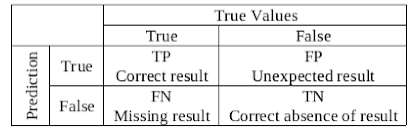
\includegraphics[width=12cm]{figures/1174077/2/cm.png}
    \centering
    \caption{Confusion Matrix}
\end{figure}	

\subsubsection{Jelaskan bagaimana K-fold cross validation bekerja dengan gambar ilustrasi contoh buatan sendiri.}
\hfill\\
Cara Kerja k-fold cross validation:
\begin{itemize}
	\item Total instance dibagi menjadi N bagian.
	\item Fold yang pertama adalah bagian pertama menjadi data uji (testing data) dan sisanya menjadi training data.
	\item Lalu hitung akurasi berdasarkan porsi data tersebut dengan menggunakan persamaan.
	\item Fold yang kedua adalah bagian kedua, yang menjadi data uji(testing data)dan sisanya training  data.
	\item Kemudian hitung akurasi berdasarkan porsi data tersebut.
	\item Dan seterusnya hingga habis mencapai fold ke-K.
	\item Terakhir hitung rata-rata akurasi K buah.
\end{itemize}
\begin{figure}[H]
    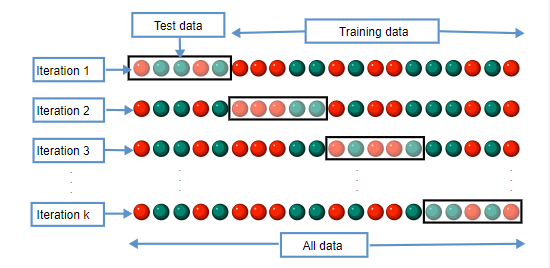
\includegraphics[width=8cm]{figures/1174077/2/kf.png}
    \centering
    \caption{K-Fold Validation}
\end{figure}

\subsubsection{Jelaskan Apa itu decision tree dengan gambar ilustrasi contoh buatan sendiri.}
\hfill\\
Decision Tree merupakan sebuah struktur yang menentukan keputusan dan setiap konsekuensinya. Hasil dari setiap struktur biasanya menggunakan jawaban (True dan False) atau cabang lain yang akan menjadi pohon selanjutnya. Setiap keputusan diantaranya akan membandingkan kondisi yang diberikan kepada struktur untuk dibandingkan kondisi apa saja yang sudah didapat pada sistem tersebut.
\begin{figure}[H]
    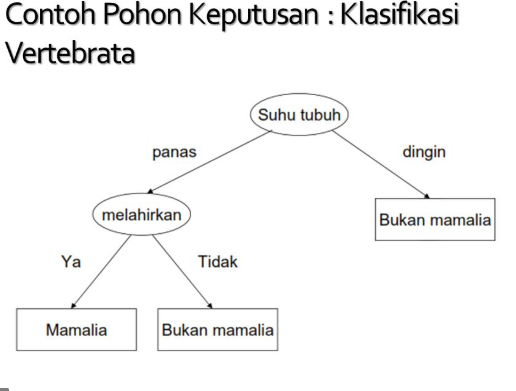
\includegraphics[width=8cm]{figures/1174077/2/dt.png}
    \centering
    \caption{Decision Tree Hewan Vertebrata}
\end{figure}


\subsubsection{jelaskan apa itu information gain dan entropi dengan gambar ilustrasi buatan sendiri.}
\hfill\\
\begin{enumerate}
	\item information Gain
	\hfill\\
	Information Gain merupakan total data yang didapat dari data - data acak yang data tersebut akan digunakan untuk analisis data lainnya. Information Gain ini digunakan pada decision tree sebagai label setiap aksi - aksi yang perlu dinilai validasinya. 
\begin{figure}[H]
    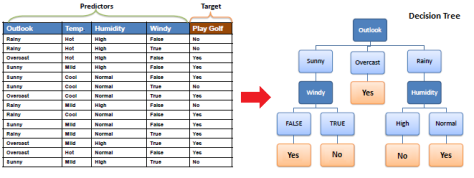
\includegraphics[width=12cm]{figures/1174077/2/ig.png}
    \centering
    \caption{information gain}
\end{figure}

	\item Entropi
	\hfill\\
	Entropi merupakan pengukuran sebuah data dan validnya data tersebut untuk dapat digunakan sebagai informasi yang akan dimasukkan ke Information Gain. Entropi menilai sebuah obyek berdasarkan kebutuhan di dunia nyata dan pengaruh pada sistem yang akan digunakan.
\begin{figure}[H]
    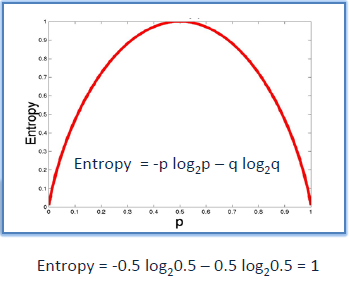
\includegraphics[width=8cm]{figures/1174077/2/e.png}
    \centering
    \caption{Entropi}
\end{figure}
\end{enumerate}



\subsection{Praktek}
Tugas anda adalah, dataset ganti menggunakan student-mat.csv dan mengganti semua nama variabel dari kode di bawah ini dengan nama-nama makanan (NPM mod 3=0), kota (NPM mod 3=1), buah (NPM mod 3=2)
\lstinputlisting[firstline=8, lastline=9]{src/1174077/2/1174077.py} 

\subsubsection{Nomor 1}
\hfill\\
\lstinputlisting[firstline=12, lastline=14]{src/1174077/2/1174077.py}
\begin{figure}[H]
\centerline{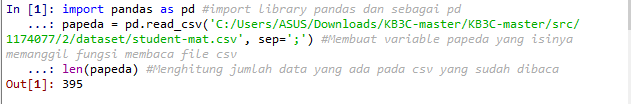
\includegraphics[width=10cm]{figures/1174077/2/p1.png}}
\caption{Nomor 1}
\label{labelgambar}
\end{figure}

\subsubsection{Nomor 2}
\hfill\\
\lstinputlisting[firstline=16, lastline=20]{src/1174077/2/1174077.py}
\begin{figure}[H]
\centerline{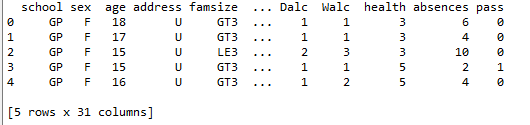
\includegraphics[width=10cm]{figures/1174077/2/p2.png}}
\caption{Nomor 2}
\label{labelgambar}
\end{figure}

\subsubsection{Nomor 3}
\hfill\\
\lstinputlisting[firstline=22, lastline=27]{src/1174077/2/1174077.py}
\begin{figure}[H]
\centerline{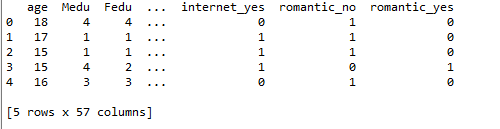
\includegraphics[width=10cm]{figures/1174077/2/p3.png}}
\caption{Nomor 3}
\label{labelgambar}
\end{figure}

\subsubsection{Nomor 4}
\hfill\\
\lstinputlisting[firstline=29, lastline=47]{src/1174077/2/1174077.py}
\begin{figure}[H]
\centerline{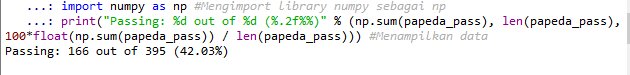
\includegraphics[width=10cm]{figures/1174077/2/p4.png}}
\caption{Nomor 4}
\label{labelgambar}
\end{figure}

\subsubsection{Nomor 5}
\hfill\\
\lstinputlisting[firstline=49, lastline=53]{src/1174077/2/1174077.py}
\begin{figure}[H]
\centerline{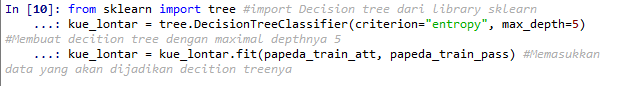
\includegraphics[width=10cm]{figures/1174077/2/p5.png}}
\caption{Nomor 5}
\label{labelgambar}
\end{figure}

\subsubsection{Nomor 6}
\hfill\\
\lstinputlisting[firstline=56, lastline=63]{src/1174077/2/1174077.py}
\begin{figure}[H]
\centerline{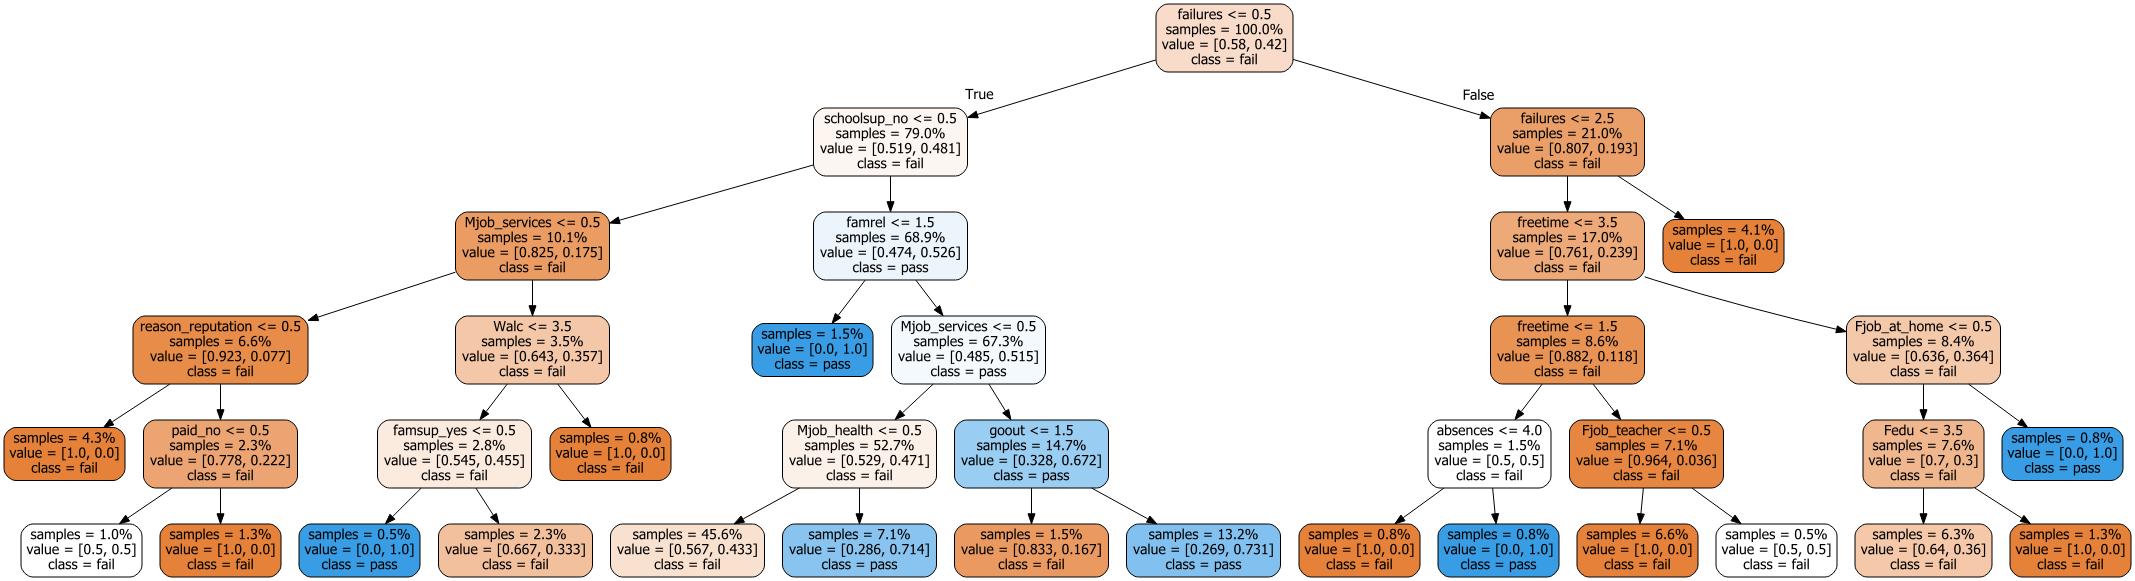
\includegraphics[width=10cm]{figures/1174077/2/p6.png}}
\caption{Nomor 6}
\label{labelgambar}
\end{figure}

\subsubsection{Nomor 7}
\hfill\\
\lstinputlisting[firstline=66, lastline=70]{src/1174077/2/1174077.py}
\begin{figure}[H]
\centerline{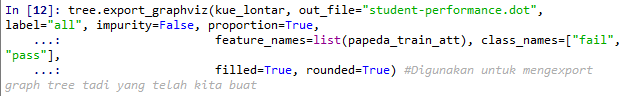
\includegraphics[width=10cm]{figures/1174077/2/p7.png}}
\caption{Nomor 7}
\label{labelgambar}
\end{figure}

\subsubsection{Nomor 8}
\hfill\\
\lstinputlisting[firstline=73, lastline=74]{src/1174077/2/1174077.py}
\begin{figure}[H]
\centerline{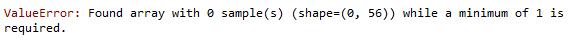
\includegraphics[width=10cm]{figures/1174077/2/p8.png}}
\caption{Nomor 8}
Error dikarenakan tidak ada sample data ditemukan
\label{labelgambar}
\end{figure}

\subsubsection{Nomor 9}
\hfill\\
\lstinputlisting[firstline=77, lastline=81]{src/1174077/2/1174077.py}
\begin{figure}[H]
\centerline{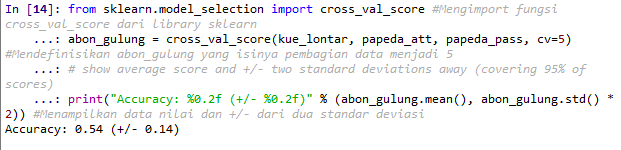
\includegraphics[width=10cm]{figures/1174077/2/p9.png}}
\caption{Nomor 9}
\label{labelgambar}
\end{figure}

\subsubsection{Nomor 10}
\hfill\\
\lstinputlisting[firstline=84, lastline=88]{src/1174077/2/1174077.py}
\begin{figure}[H]
\centerline{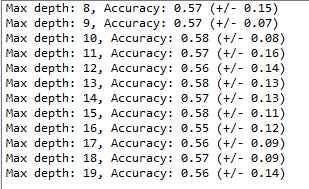
\includegraphics[width=10cm]{figures/1174077/2/p10.png}}
\caption{Nomor 10}
\label{labelgambar}
\end{figure}

\subsubsection{Nomor 11}
\hfill\\
\lstinputlisting[firstline=91, lastline=102]{src/1174077/2/1174077.py}
\begin{figure}[H]
\centerline{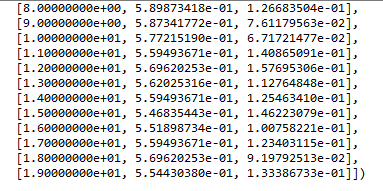
\includegraphics[width=10cm]{figures/1174077/2/p11.png}}
\caption{Nomor 11}
\label{labelgambar}
\end{figure}

\subsubsection{Nomor 12}
\hfill\\
\lstinputlisting[firstline=105, lastline=109]{src/1174077/2/1174077.py}
\begin{figure}[H]
\centerline{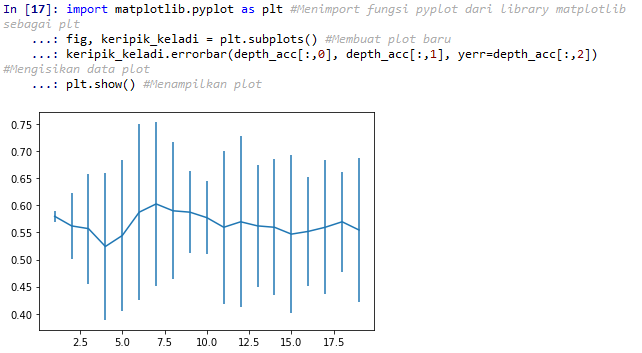
\includegraphics[width=10cm]{figures/1174077/2/p12.png}}
\caption{Nomor 12}
\label{labelgambar}
\end{figure}

\subsection{Penanganan Error}
\subsubsection{Error}
\hfill\\
\begin{enumerate}
\item ModuleNotFoundError

\begin{figure}[H]
\centerline{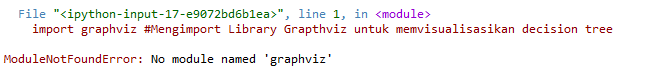
\includegraphics[width=10cm]{figures/1174077/2/error1.png}}
\caption{ModuleNotFoundError}
\label{labelgambar}
\end{figure}
\end{enumerate}

\subsubsection{Solusi}
\begin{enumerate}
\item Intall library Graphviz dengan cara download graphviz di google

setelah instalasi buka anaconda prompt sebagai admin lalu mengetikkan
\begin{lstlisting}
conda install graphviz
\end{lstlisting} 
\end{enumerate}

\subsection{Bukti Tidak Plagiat}
\hfill\\
\begin{figure}[H]
\centerline{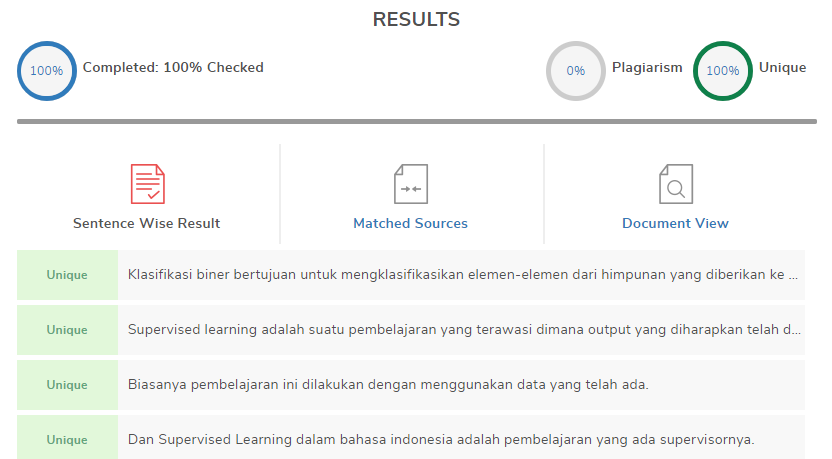
\includegraphics[width=10cm]{figures/1174077/2/plagiat.png}}
\caption{Bukti Tidak Plagiat}
\label{labelgambar}
\end{figure}